\section{AphraFinance}
\label{sec:aphrafinance}
\aphra is a scriptable financial protocol designed to operate a peg stability module for algorithmic stablecoins.
We use revenue from cashflow-generating assets and fees generated from peg arbitrage supported by protocol-owned liquidity (POL) to make the protocol functional.\cite{aphra-finance}
Our main mission is to become a ``black hole'' for decentralized liquidity that is used to regulate stablecoin pegs.
Furthermore, a positive market action is created as more and more assets are taken out of circulation. 
POL anchors those pegs by prohibiting market manipulation and economic attacks through adjustment of price fluctuations using automatized workflow actions.
The \aphra engine implements automatized workflows that consist of economic actions each propagating the actual workflow-state to the next one.
These actions are authorized contracts that live on-chain and are able to be executed in single calls using \textit{multisig} procedures within the modified \textit{weiroll} VM.\cite{weirollvm}
The protocol is bootstrapped as a continuous integration platform similar to, \textit{e.g.}, Amazon Web Services, where experts are able to implement financial strategies in terms of directed acyclic graph\cite{thulasiraman2011} workflows.
Authorization, feasibility, and ecosystem health are cross-checked by the \aphra scoring mechanism obtained through trusted participants that validate runs by providing trust scores in a similar way to, \textit{e.g.}, oracles.
Execution of workflows with high-enough trust scores will be performed while low trust-score workflows will not be executed.
Next, we describe the structure of the \aphra engine and the underlying continuous integration platform as a combined and simplified ecosystem representation:

\begin{figure}[p]
    \vspace*{-2cm}
    \makebox[\linewidth]{
        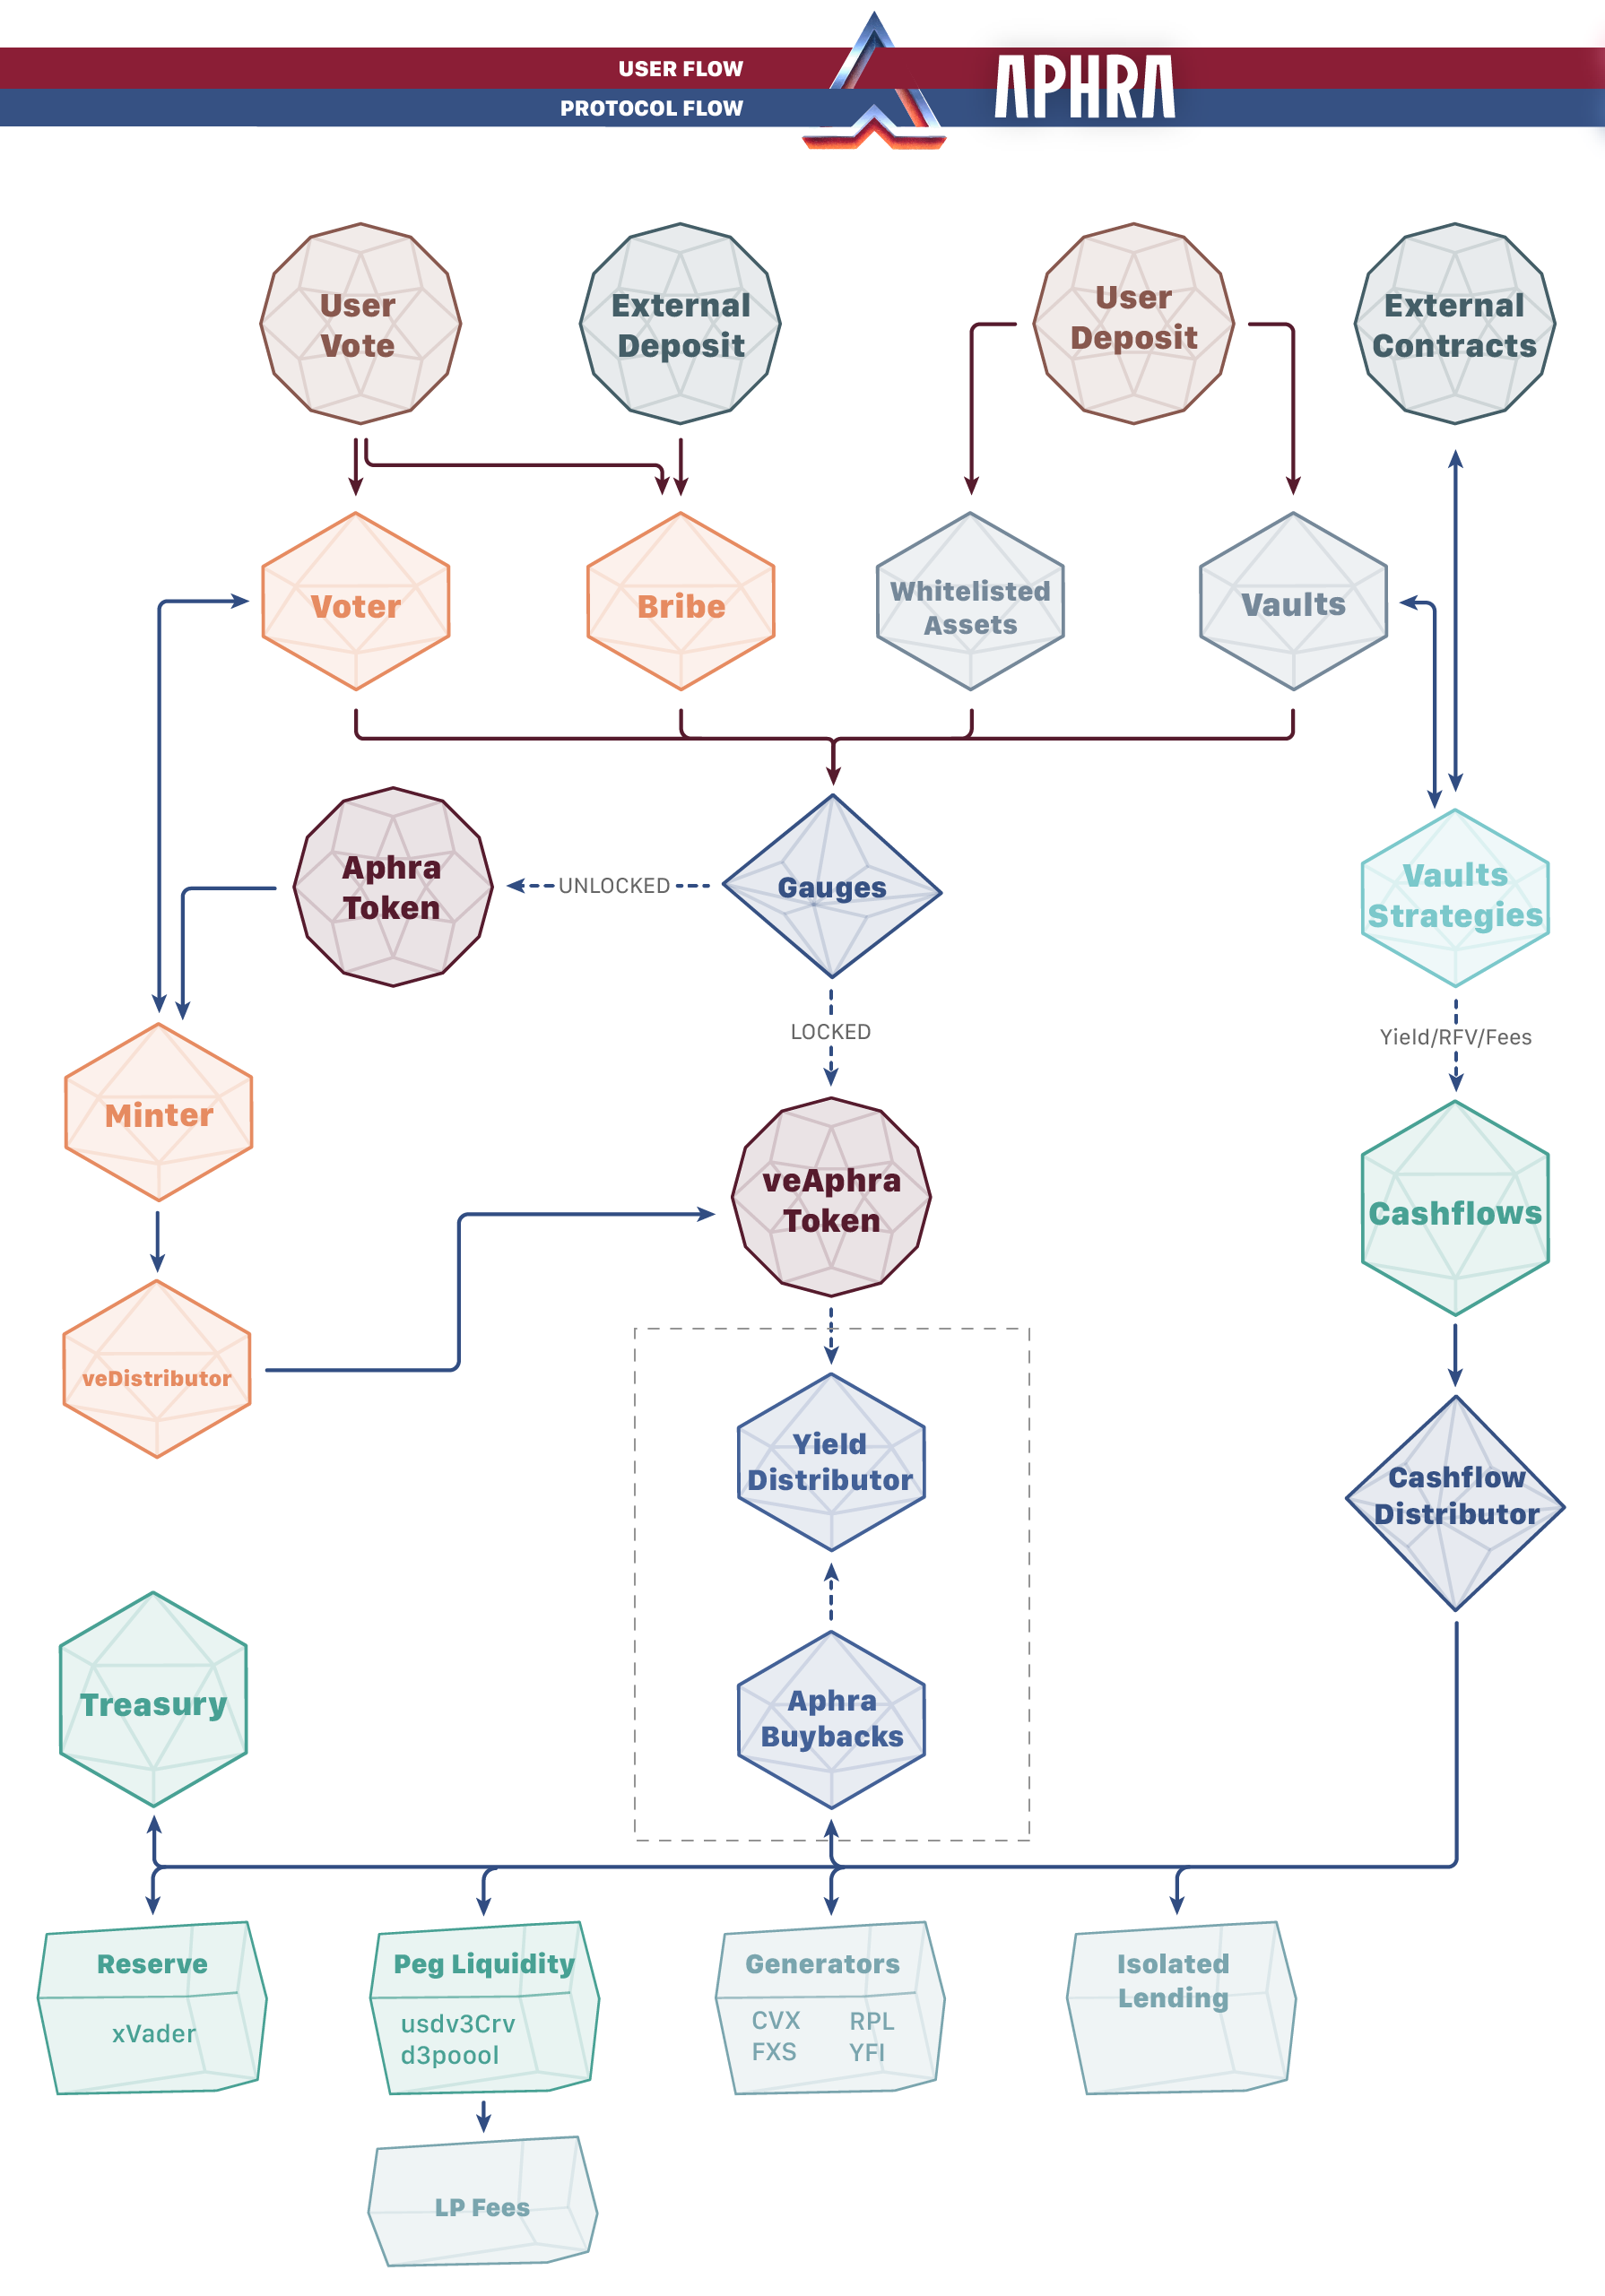
\includegraphics[width=1.3\linewidth]{figures/AphraEngine.png}
    }
    \caption{Flowchart diagram of the \aphra ecosystem from the perspective of end-users, who provide liquidity and can help shape the DAO through voting rights as obtained \textit{via} vote-escrowed \aphra tokens.}
    \label{fig:ae-flow}
\end{figure}

\aphra vaults allow the end-user to deposit liquidity within expert yield aggregator strategies -- more details are given in section\,\ref{subsec:aphra-yield-farming}.
Another stake vector is provided by means of white-listed crypto assets, where the end-user can provide liquidity through crypto assets that are used within yield farming strategies like peg arbitrage.
The end-user obtains 20\% of the generated revenue and is entitled to obtain ve\aphra from weekly inflation.
The usage is measured with gauges, which show how much an end-user is providing in liquidity.
Each gauge is associated with a weight that determines how much of the inflation will be received by this liquidity gauge.
All weights add up to unity and we calculate the inflation each week as discussed in section\,\ref{subsec:ve-mechanism} until the unlock vote passes (see section\,\ref{subsec:dao-activation}).\\[-1em]

Inflation is created by the \aphra minter and paid out to the liquidity gauges according to the pre-voted weights by the veDistributor.
After the DAO activation, the inflation rate is dynamically defined with respect to ve-locked circulating supply (see section\,\ref{subsec:ve-mechanism}).
ve\aphra holders decide through voting how the gauges inflation weights should be adjusted.
Voting rights can also be acquired, which means that ve\aphra holders can pass on their voting rights to others by receiving financial incentives through voting bribes.
Bribes thus allow the ve\aphra holder to build an additional passive revenue stream.
After the distribution scheme is determined, inflation will be distributed to gauges liquidity providers with a minimum locking period.
At this point it should also be said that there is a dilution protection for ve\aphra holders, which ensures that ve-locks increase based on the existing inflation.\\[-1em]

Initial cashflow is generated by the remaining 80\% revenue as obtained by \aphra yield farming strategies (see section\,\ref{subsec:aphra-yield-farming}).
The integrated cashflow distributor gauge allocates liquidity to the different key areas of the ecosystem in order to maximize project-owned liquidity while helping our partner networks in the best possible way.
Key areas of the ecosystem are: I) a protocol reserve as locked in x\vader tokens, II) peg liquidity through \usdv3\crv and a decentralised stablecoin pool consisting of three different algorithmic stablecoins (\usdv,\cite{vader} \bean,\cite{bean} and \frax\cite{frax}), III) cashflow generating assets (\textit{e.g.}, \crv,\cite{curve} \fxs,\cite{frax} \rpl,\cite{rocket-pool} or \yfi\cite{yearn-finance}), and IV) an isolated lending market. 
Initial priority is the development of project-owned reserves and the setup of peg liquidity since we see those points as base pillars of the ecosystem.
Once a reliable source of cashflow has established through stablecoin peg arbitrage, the future health of the \aphra DAO is consolidated.
As soon as we reach a reasonable reserve of POL (45--50 million), another key area of the protocol gets activated -- an isolated lending market.
This will enable the development of new strategies by means of the recently published YieldBox.\cite{yieldbox,boringcrypto}
More details about the isolated lending market follow in an upcoming version.

\subsection{Vote-escrowed mechanism}
\label{subsec:ve-mechanism}
Standard vote-escrowed (ve) rules enables the end-user to lock a base token into the ve-contract for a period of one week to up to four years.
Those locks are, however, not transferable and thus bound to one address.
Holder of ve-tokens vote on the destribution of inflation and hence which liquidity pools should be incentivized.
Three changes to this standard procedure have been suggested\cite{andre-conje} and implemented within the ve\aphra model: First, inflation is dynamically determined with respect to the amount of ve-locked circulating supply, which will be the active mechanism after the DAO activation.
Before that the inflation rate $\theta$ is set to a value of 625,000.

\vskip1em
\begin{figure}
    \centering
    \pgfplotsset{scaled y ticks=false}
    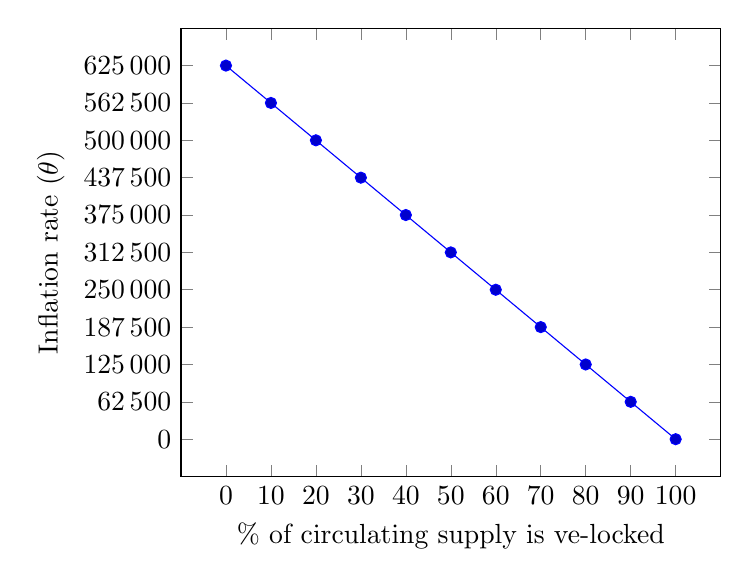
\begin{tikzpicture}
    \begin{axis}[
    ytick={625000,562500,500000,437500,375000,312500,250000,187500,125000,62500,0},
    yticklabels = {625\,000,562\,500,500\,000,437\,500,375\,000,312\,500,250\,000,187\,500,125\,000,62\,500,0},
    xtick={0,10,20,30,40,50,60,70,80,90,100},
    xlabel={\% of circulating supply is ve-locked},ylabel={Inflation rate ($\theta$)}]
    \addplot coordinates {
      (0, 625000)
      (10, 562500)
      (20, 500000)
      (30, 437500)
      (40, 375000)
      (50, 312500)
      (60, 250000)
      (70, 187500)
      (80, 125000)
      (90, 62500)
      (100, 0)
    };
    \end{axis}
    \end{tikzpicture}
    \caption{Inflation rate is depending on ve-locked circulating supply.}
    \label{fig:ve-circulating-supply}
\end{figure}
\vskip1em
The inflation is calculated according to equation\,\ref{eq:inflation}, where we use the inflation rate $\theta$, the weekly emission $\alpha_w$, the circulating supply (CS), and the total supply (TS).
The weekly emission will decay at a rate of two percent per week.
An example clarifies how we calculate the inflation:
Starting with an inflation constant of 625,000, a weekly emission constant of 98, a CS of 8,000,000, and a TS of 29,500,000 we obtain the following inflation
\begin{equation}
    \text{Inflation} = \frac{\theta\,\alpha_{\text{w}}\,\text{CS}}{100\,\text{TS}} = \frac{625,000 \times 98 \times 8,000,000}{100 \times 29,500,000} = 166,101\,\frac{41}{59}.
    \label{eq:inflation}
\end{equation}
Second, all ve-lockers increase their holdings proportional to the inflation.
Following the example given above the weekly inflation rate is 0.54\%.
Our modification will ensure that ve-lockers will never be diluted, as such, their holdings increase by 0.54\%.
Last, ve-lockers are represented as non-fungible token\cite{wang2021_2,ante2021} (NFT), which allows a single address to have multiple locks with different locking periods at the same time.
This further allows ve-locks to be traded on secondary markets, which solves the capital inefficiency problem of standard ve-tokens.
The maximum locking time is shortened from four years to two years (see section\,\ref{subsec:dao-activation}).
We present next how \aphra vaults help the end-user to generate yields and the protocol to build up a healthy DAO ecosystem.

\subsection{Aphra yield farming}
\label{subsec:aphra-yield-farming}
In the DeFi space, there are many projects that give out rewards to their end-users for interacting with their platforms.
One example is staking tokens on a platform, which in turn can increase the total value locked for that project.
Typically, liquidity pool tokens are used for this purpose, as many projects issue rewards in return for users providing the liquidity needed to run the platform, which is commonly referred to as yield farming.
For end-users with limited means, yield farming can be prohibitively expensive due to the high transaction costs of claiming rewards. 
To address this problem, so-called yield aggregator contracts have been developed to pool the funds used and allow users to optimise their return.\cite{cousaert2021}\\[-1em]

A yield aggregator is a set of smart contracts that pools invested funds, and reinvests them in an array of yield-producing products or services through interacting with their respective protocols. 
The level of aggregation offered by yield aggregators usually has a number of advantages. 
First, investors do not have to actively put together their own strategy, but can use developed expert strategies and transform their investment strategy from an active to a passive approach without requiring extensive knowledge of the underlying protocols and infrastructures.
Secondly, since cross-protocol transactions take place \textit{via} a smart contract, capital shifts are performed automatic, removing the need for the investor to transfer funds manually between protocols.
Finally, because funds are pooled in a strategy contract, the gas costs are socialized, resulting generally in fewer and thus lower interaction costs.\\[-1em]

AphraFinance offers the end-user to participate in yield aggregator strategies. 
Locked provided liquidity is allocated to be used in strategies to, \textit{e.g.}, peg arbitrage algorithmic stablecoins (see section \ref{sec:peg_maintenance}).
This allows both the stablecoin community and the end-user to benefit from AE strategies.
Beneath obtaining ve\aphra inflation as reward, 20\% of the yield farming aggregator revenue is entitled to the liquidity provider, while 80\% are retained as fees by the protocol.

\subsection{Tokenomics}
\label{subsec:tokenomics}
The total supply of the \aphra token is set at 100 million tokens and we show its total distribution in the pie chart below.

% Tikz pie chart style defined in "config.tex"
% Note that chart has a total of 100%
% Each piece takes some %, so in the end we need to add up to 100
% Example allocation below, colors are defined within "colors" below
% Define piece by "%/Name" below in "3d pie chart"
% Height, radius, and font can be defined as well. Enjoy!
\vskip1em
\begin{figure}[ht!]
    \centering
    \begin{tikzpicture}[font=\sffamily]
     \path[
     3d pie chart/.cd,
     radius=2.5cm,
     h=1cm,
     % Custom colors defined in "config.tex"
     colors={
     "ticklemepink", % Deposits
     "ufogreen",     % Airdrop
     "darkcyan",     % DAO
     "gray",         % Furure staff
     "vanilla",      % Founder & team
     }
     ] pic{
     3d pie chart={
     60/Aphra deposits,
     3/Airdrop,
     22/DAO,
     9/Future staff,
     6/Founder and Team}
     };
    \end{tikzpicture}
    \label{fig:tokenomics}
    \caption{Total \aphra token distribution.}
\end{figure}
\vskip1em
15 million tokens or 15\% of \aphra's token supply is allocated to the AphraFinance team with 6\% getting allocated towards the existing team and 9\% being reserved for future team members.
The existing team receives 6\% of the \aphra token supply with 2\% being reserved for the founder and 1\% being reserved for every other team member, where allocation is given to 100\% in ve\aphra.
The allocations for future team members will be decided on a case by case basis as the project and the value of the token evolve.
Current and future AphraFinance team members receive half of their allocation in ve\aphra with a 2 year locking period and the other half of their allocation in the form of \aphra base tokens.
There exist a technical council that is responsible for hiring new team members (see section\,\ref{subsec:dao-governance}).\\[-1em]

3\% of \aphra's supply which equates to 3 million tokens will be reserved for the airdrop recipients and will be emitted in the form of ve\aphra with a 6 month lock over the course of 6 months.
Eligible airdrop participants have staked \vader tokens before the snapshot \textsc{Ethereum} block \href{https://etherscan.io/block/13925000}{\textsc{13925000}}, staked tokens in a BeanstalkFarms SILO, SOW'ed\cite{bean}, or staked \fxs tokens before the snapshot \textsc{Ethereum} block \href{https://etherscan.io/block/14005000}{\textsc{14005000}}.\cite{frax}
All airdrop addresses (5,896 participants) are shared separately.\cite{aphradrop}
Airdrop recipients can claim their airdrop whenever they want, however, the unvested portion of their airdrop will be forfeited and redistributed to the addresses that have not claimed yet.\\[-1em]

60\% of the token supply which equates to 60 million tokens is scheduled to be emitted into \aphra depositors as incentives, where a certain amount is reserved for vaults.
The purpose of this is to incentivise market actors to take actions that lead to the growth of AphraFinance over the long term.
In a future update, token emissions can be adjusted in real time between different stablecoin vaults in case of a peg dislocation with the aim of attracting market actions that can restore the peg of a specific stablecoin if needed.
In the future, vault deposits can be represented with yield bearing \textsc{erc20} tokens that can be used as collateral into different DeFi protocols. 
Below is the schedule of emissions towards \aphra deposits:
\vskip1em
\begin{figure}
    \centering
    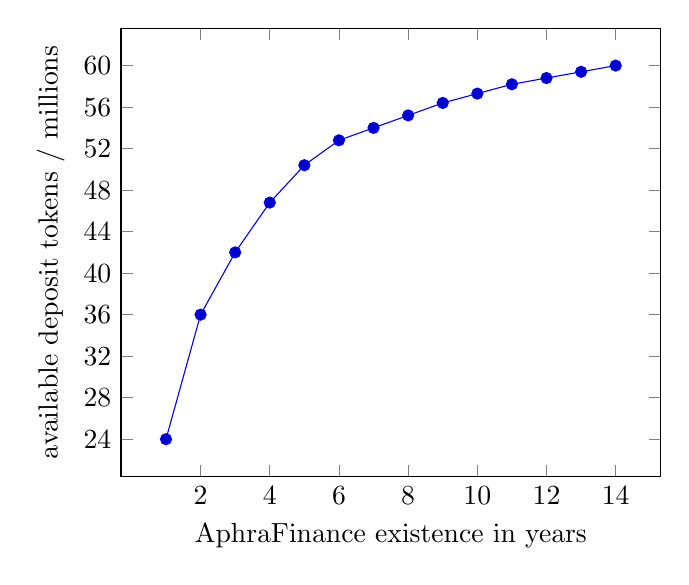
\begin{tikzpicture}
    \begin{axis}[ytick={24,28,32,36,40,44,48,52,56,60}, xtick={2,4,6,8,10,12,14},xlabel={AphraFinance existence in years},ylabel={available deposit tokens / millions}]
    \addplot coordinates {
      (1, 24.0)
      (2, 36.0)
      (3, 42.0)
      (4, 46.8)
      (5, 50.4)
      (6, 52.8)
      (7, 54.0)
      (8, 55.2)
      (9, 56.4)
      (10, 57.3)
      (11, 58.2)
      (12, 58.8)
      (13, 59.4)
      (14, 60.0)
    };
    \end{axis}
    \end{tikzpicture}
    \caption{Emission of \aphra deposit tokens within the upcoming 14 years.}
    \label{fig:deposit-emission}
\end{figure}
\vskip1em
By having a long term emissions schedule, AphraFinance attracts capital flows in order to establish itself with the aim of keeping that capital by benefiting all participants of its ecosystem through the results of its actions.
After the endpoint of AphraFinance's emission schedule, the DAO can arrive to the decision of directing part of AphraFinance profits into the buyback of \aphra tokens on the open market in order to distribute them to depositors as rewards.\\[-1em]

22\% of the \aphra supply which equates to 22 million tokens is reserved for the DAO treasury and is granted through a 14 year emissions schedule that follows the issuance rate decrease that is established by the deposits emission schedule as described above.
The DAO emission scheme is presented below:
\vskip1em
\begin{figure}
    \centering
    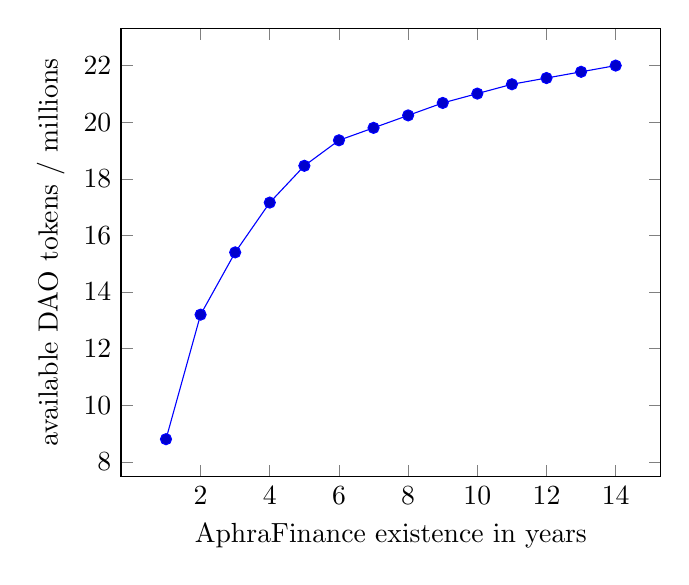
\begin{tikzpicture}
    \begin{axis}[ytick={8,10,12,14,16,18,20,22}, xtick={2,4,6,8,10,12,14},xlabel={AphraFinance existence in years},ylabel={available DAO tokens / millions}]
    \addplot coordinates {
      (1,  8.8)
      (2, 13.2)
      (3, 15.4)
      (4, 17.16)
      (5, 18.46)
      (6, 19.36)
      (7, 19.80)
      (8, 20.24)
      (9, 20.68)
      (10, 21.01)
      (11, 21.34)
      (12, 21.56)
      (13, 21.78)
      (14, 22.00)
    };
    \end{axis}
    \end{tikzpicture}
    \caption{Emission of \aphra DAO tokens within the upcoming 14 years.}
    \label{fig:dao-emission}
\end{figure}
\vskip1em
The DAO  is tasked with making decisions in regards to the optimal use of treasury funds with the end goal of advancing AphraFinance and its ecosystem partners forward.\\[-1em]

Treasury funds can be used for the following purposes:
\begin{itemize}
    \item[\textbf{1}] Grants for research and development that can lead to the further development of AphraFinance and its ecosystem.
    \item[\textbf{2}] Execution of treasury swaps with other entities for strategic purposes.
    \item[\textbf{3}] Funding the seed and investment rounds of projects that can further advance AphraFinance and its ecosystem partners through innovative offerings.
    \item[\textbf{4}] Investing into assets that can be beneficial to AphraFinance and its ecosystem from a strategic perspective.
    \item[\textbf{5}] Offering of \aphra tokens into the market through the sale of bonds.
    \item[\textbf{6}] Security audits of smart contracts.
    \item[\textbf{7}] Continuous funding of the Coordinape\cite{coordinape} circle in order to reward productive engagement from the AphraFinance community (\textit{vide infra}).
    \item[\textbf{8}] Any other expense that is deemed to be essential or worthwhile for the advancement or operations of AphraFinance.
\end{itemize}


\subsection{DAO: Activation}
\label{subsec:dao-activation}
In order for the AphraFinance DAO to be activated and the \aphra token to become tradeable, a vote with a duration of 7 days will be enacted requiring 15,000,000 tokens in favor. 
In case of failing the proposal to pass, the vote can be reenacted every 200,000 blocks until there is agreement within the community.
With the activation of the DAO, an additional vault for \aphra/\usdv liquidity pools will be introduced with the aim of incentivising market actors for the provision of liquidity into decentralised exchanges.
For the first 6 months of the emission schedule all rewards will be provided in the form of ve\aphra with the locking applying for a duration of 6 months. 
After the DAO activation, all the rewards will be provided in the form of the base \aphra token with the option of locking laying in the hands of each individual participant.\\[-1em]

\aphra token holders can lock their tokens for up to two years in order to participate in the DAO and the value it generates.
The exact \aphra to ve\aphra exchange rate is dependent on the locking period as seen below:

\vskip1em
\begin{figure}
    \centering
    \begin{tikzpicture}
    \begin{axis}[ytick={0.25, 0.50, 0.75, 1.00}, xtick={6,12,18,24}, yticklabels = {0.25, 0.50, 0.75, 1.00},xlabel={\aphra locking in months},ylabel={ve\aphra / \aphra \, rate}]
    \addplot coordinates {
      (6, 0.25)
      (12, 0.50)
      (18, 0.75)
      (24, 1.00)
    };
    \end{axis}
    \end{tikzpicture}
    \caption{Exchange rate of ve\aphra for \aphra depends on chosen locking period.}
    \label{fig:aphra-veaphra}
\end{figure}
\vskip1em

For a locking period of 6 months, one \aphra token will be exchanged to 0.25 ve\aphra.
An increase of locking time will increase the exchange rate for ve\aphra tokens.
The maximum amount is obtained for a locking period of 24 months, where one \aphra tokens is exchanged to one ve\aphra token.
Vote locked \aphra can be represented as NFT giving \aphra vote lockers the ability of having multiple locks inside a wallet for different quantities and time horizons.
The representation of vote locked positions as \textsc{NFTs} also creates the capability of enabling a vote market inside AphraFinance itself thus creating another source of yield for ve\aphra positions.
Furthermore, ve\aphra holders will be able to participate in the DAO decision making process regardless of the size of their holdings.
For the submission of proposals to the DAO, a minimum of 2500 ve\aphra tokens will be required.
Submissions will be published on the Snapshot\cite{aphra-snapshot} platform (see section \ref{subsec:dao-governance}).\\[-1em]

As AphraFinance produces cashflow those assets will be used as follows: First, we provide another source of funding for the DAO treasury outside of the emissions of our native token.
Second, we accumulate strategic cashflow producing assets with voting rights (\textit{e.g.}, \cvx,\cite{convex} \vader,\cite{vader} or \fxs\cite{frax}) and compound these positions while a percentage of the profits can be directed towards ve\aphra holders.
Lastly, direct part of protocol profits is redirected towards ve\aphra holders through the buyback and distribution of native tokens or in other ways that can be voted on by the DAO.
The DAO furthermore adjusts the ratios of the allocations towards each one of the specified strategies however it sees fit.
Once credibility has been established, AphraFinance can take on higher risk activities like providing credit lines to other DAOs.

\subsection{DAO: Governance}
\label{subsec:dao-governance}
One of the most immediate challenges for decentralized communities is how to address governance.
Managing collective decision making to optimize resources and operations plays a critical role.
Governance, however, requires a significant coordination effort stemming from the need to involve network participants in voting on every decision.
This coordination effort can be radically reduced in decentralized networks where smart contracts enable participants to govern cooperatively.
DAOs run almost entirely by code and refer to collections of people that come together with aligned incentives and interests.\\[-1em]

Within the DAO, we have two councils: First, a technical council that will come up with suggestions on improving the ecosystem on a technical level and the hiring process of new personal (see ``Hire staff'' below).
Second, a treasury council that will come up with suggestions on asset management and asset curation (see ``Risk management'' and ``Asset curation'' below).
All suggestions will be released in transparent proposals that have to go through a community election where we decide collectively on important changes by using voting power that has been transferred to holders of the ve\aphra governance token.
All proposals will be published on the Snapshot\cite{aphra-snapshot} platform.\\[-1em]

Incentives are critical to governance because otherwise there is little reason for community members to invest time, money, or energy in managing or improving the ecosystem.
Therefore, we established a reward system to acknowledge active members in the community for their contributions (see ``Community rewards'' below).
Note that we actively reward good ideas and suggestions that will lead to the improvement of the ecosystem.
We list in the following essential subjects that are crucial to the success of the DAO:

\paragraph{\textbf{Collective asset management}}
Initial capital is provided in the form of governance tokens held by the DAO smart contract and assets used to purchase governance tokens.
For example, if the DAO begins minting 1,000 governance tokens and sells 500 of them to genesis members for 100 \eth, then the initial treasury consists of 500 governance tokens and 100 \eth. 
However, as the DAO grows in terms of user base or accumulated cash-flows, it becomes important for the DAO to manage this capital similar to a business.

\paragraph{\textbf{Risk management}}
The balance sheet of the DAO can consist of risky assets.
Therefore, managing currency risk is very important to ensure that future operations can be funded.
These assets are intended to be used to fund development, audits, insurance, and for spending on user growth and acquisition. 
To achieve these goals, we must manage the treasury to meet specific metrics or key performance indicators (KPIs).
Quantitative tools are useful in enabling the community to visualize and make DAO members understand the risk of the DAO in relation to market conditions.
This creates more transparency on the risk level of a DAO treasury and allows the community to update the treasury composition to meet specific KPIs.

\paragraph{\textbf{Asset curation}}
The DAO governance token is used for voting on adding or removing assets. 
This is because a number of parameters must be chosen for each asset - margin requirements, yield curves, insurance costs - and the decisions are critical to the security of the ecosystem. 

\paragraph{\textbf{Hire staff}}
Once the DAO has a large enough community and sufficient assets, it is important to hire people who can take care of maintenance, communication, and administrative tasks full time.
The DAO must, however, be careful not to create "active participants" that token holders could rely on to increase the value of the underlying token. 
Therefore, decentralization must be kept in mind when adding service providers. 

\paragraph{\textbf{Community rewards}}
Community grants, internal salaries and special projects can be stimulated and rewarded by the community itself. 
Instead of cumbersome voting or black box committees, contributors themselves can quickly and transparently reward the value they believe has been created.
For this purpose, we have created an AphraFinance-Coordinape circle,\cite{coordinape} which enables active members to be rewarded based on their contributions.
Within the circle, each member has an amount of 100 \textsc{give} tokens that can be distributed to other members in the circle.
After each epoch (1 month), a certain amount of ve\aphra tokens will be allocated based on the amount of \textsc{give} tokens distributed.
New members can be elected by existing circle members to also participate in the distribution of rewards.
Three votes of active circle members are necessary to become a member of the AphraFinance-Coordinape circle.
Note that the amount of distributed \aphra tokens can be adjusted in the future through DAO governance.

\section{Peg maintenance}
\label{sec:peg_maintenance}
End-users rely on the maintenance of the peg for predictable value transfer. 
Hence the maintenance of the peg should be used as the primary indicator of value.
However, in the case of algorithmic stablecoins, there are a number of other relevant parties from whose perspective the value of the stablecoin ecosystem can be assessed.
There is a significant profit opportunity for arbitrageurs and speculators exposed to the stablecoin and its stabilizing asset.
The theoretical loss of value due to the divergence of the peg is at least partially offset by the resulting opportunities for these parties to earn relatively low-risk returns by participating in the rebalancing process, which could optimistically be viewed as a benefit shift rather than a net loss.
Here, the end-user only suffers a loss of value from a peg deviation if he sells the stablecoin before the successful rebalancing.
Thus, the time required for rebalancing is a metric that can be used to measure the value of the stablecoin.\\[-1em]

The concept of time value of money states that assets that can be spent in the present are worth more than assets that can be spent in the future. 
Assuming that a rational end-user whose stablecoins have fallen below their peg waits until the peg is restored to spend them, and that the peg is indeed restored at some point in the future, the net present value of the stablecoins to the user decreases only as the expected time to restore equilibrium increases.
In this scenario, the magnitude of a given deviation ultimately determines value only to the extent that it affects the time required to restore equilibrium, making the latter the primary indicator of value. It should be noted, however, that this logic is not the only relevant factor, because the longer the expected rebalancing time of a stablecoin, the greater the risk that its holder will incur opportunity costs or other unavoidable costs while waiting for the peg to be restored.
There are scenarios in which opportunity costs become so large or other costs become so immediate that the end user must liquidate before rebalancing, in which case the magnitude of the deviation is likely to be as important or more important than the rebalancing time.\\[-1em]

In the following, we present our solution to minimize the rebalancing time and thus offer the end-user the possibility to cash out his value whenever it might be convenient.
We use POL, together with automated processes, to ensure that the rebalance time is kept as short as possible.
The automated processes are stored as code in the AE peg stability module (AE-PSM) and ensure that an algorithmic stablecoin maintains its peg in the long term.
At the same time, arbitrage opportunities arise, which allow us to add another source of income and thus a positive cashflow to maintain the DAO ecosystem.
In the following section, we exemplify the AE-PSM by presenting its effect on the peg of the \usdv stablecoin as released recently by the developers of the \vader protocol.

\subsection{Peg stability module: USDV example}
\label{subsec:peg_stability_module}
\vader is a liquidity protocol that combines a hybrid algorithmic-collateralized stablecoin with liquidity pools enhanced via synthetic assets.\cite{vader}
The stablecoin, \usdv, is issued by burning \vader tokens and liquidity pools use \usdv as the settlement asset.
Therefore, it is of utmost interest to the end-user that the \usdv peg is kept stable.
The AE-PSM has an API entry point (\textit{hit} function) which can be used to call methods within the module.
Pseudocode for the \textit{hit} method is given below:

\begin{lstlisting}[language={Solidity}, caption={$hit$ defines the entry point to the PSM.}]
// Get actual price, check for events,
// and payout reward in case that event happened.
function hit(uint256 amount) internal {

    // Get price information
    uint256 price = feed.getPrice();
    uint256 delta = uint256(0);
    
    // Check for possible events
    if (price >= high) {
        delta = pegDown(amount);
    } else if (price <= low) {
        delta = pegUp(amount);
    }
    
    // Payout reward
    if (delta > actionableDelta) {
        aphra.safeTransferFrom(
            address(this), address(msg.sender));
    }
}
\end{lstlisting}

If there is too much \usdv in circulation and its price is trading below the peg, then the ``pegUp'' PSM-method automatically mines \vader from existing \usdv such that there is less amount in circulation and thus the price is rebalancing back to its peg.
Pseudocode for the \textit{pegUp} method is given below:

\begin{lstlisting}[language={Solidity}, caption={$pegUp$ gets xVader from USDV.}]
// Mints Vader from USDV and stakes Vader to 
// increase xVader to bring the ratio back in line.
// Amount represents how much USDV is to be removed.
function pegUp(uint256 amount) internal {

    // USDV position in metapool, coin 0
    int128 usdv = 0;
    
    // How much USDV to remove from the pool
    uint withdraw = right.calc_withdraw(amount, usdv);
    
    // remove USDV
    right.remove_liquidity(withdraw, usdv);
    
    // Partner burn the USDV to mint Vader
    uint256 vader = vaderMinter.partnerBurn(withdraw);
    
    // Stake the Vader to increase xVader
    left.enter(vader);
}
\end{lstlisting}

On the other hand, if the price is above the peg, the \textit{pegDown} method is used.
This method burns existing \vader and \usdv is minted.
As a result, the amount of \usdv that is in circulation is increased leading to a reduction in price achieving peg stability.
Pseudocode for the \textit{pegDown} method is given below:

\begin{lstlisting}[language={Solidity}, caption={$pegDown$ gets USDV from xVader.}]
// Redeem Vader for xVader, partner mints, and then
// deposit into the pool to bring the ratio back in line.
// Amount represents how much xVader is to be removed.
function pegDown(uint256 amount) internal {

    // Hits the leave method
    left.leave(amount);
    
    // Burn all of our Vader on the PSM
    uint256 usdv = vaderMinter.partnerMinter(
        vader.balanceOf(address(this)));
    
    // Define minimum amount to stake
    uint256 min = right.calc_token_amount(
        rightPool, [usdv, 0, 0, 0], true);
    
    // Setup enforcement checks
    right.add_liquidity(rightPool, [usdv, 0, 0, 0], min);
}
\end{lstlisting}

A simplified \usdv peg rebalancing can be seen in Fig.\,\ref{fig:peg_stability}.

\vskip1em
\begin{figure}[ht!]
    \centering
    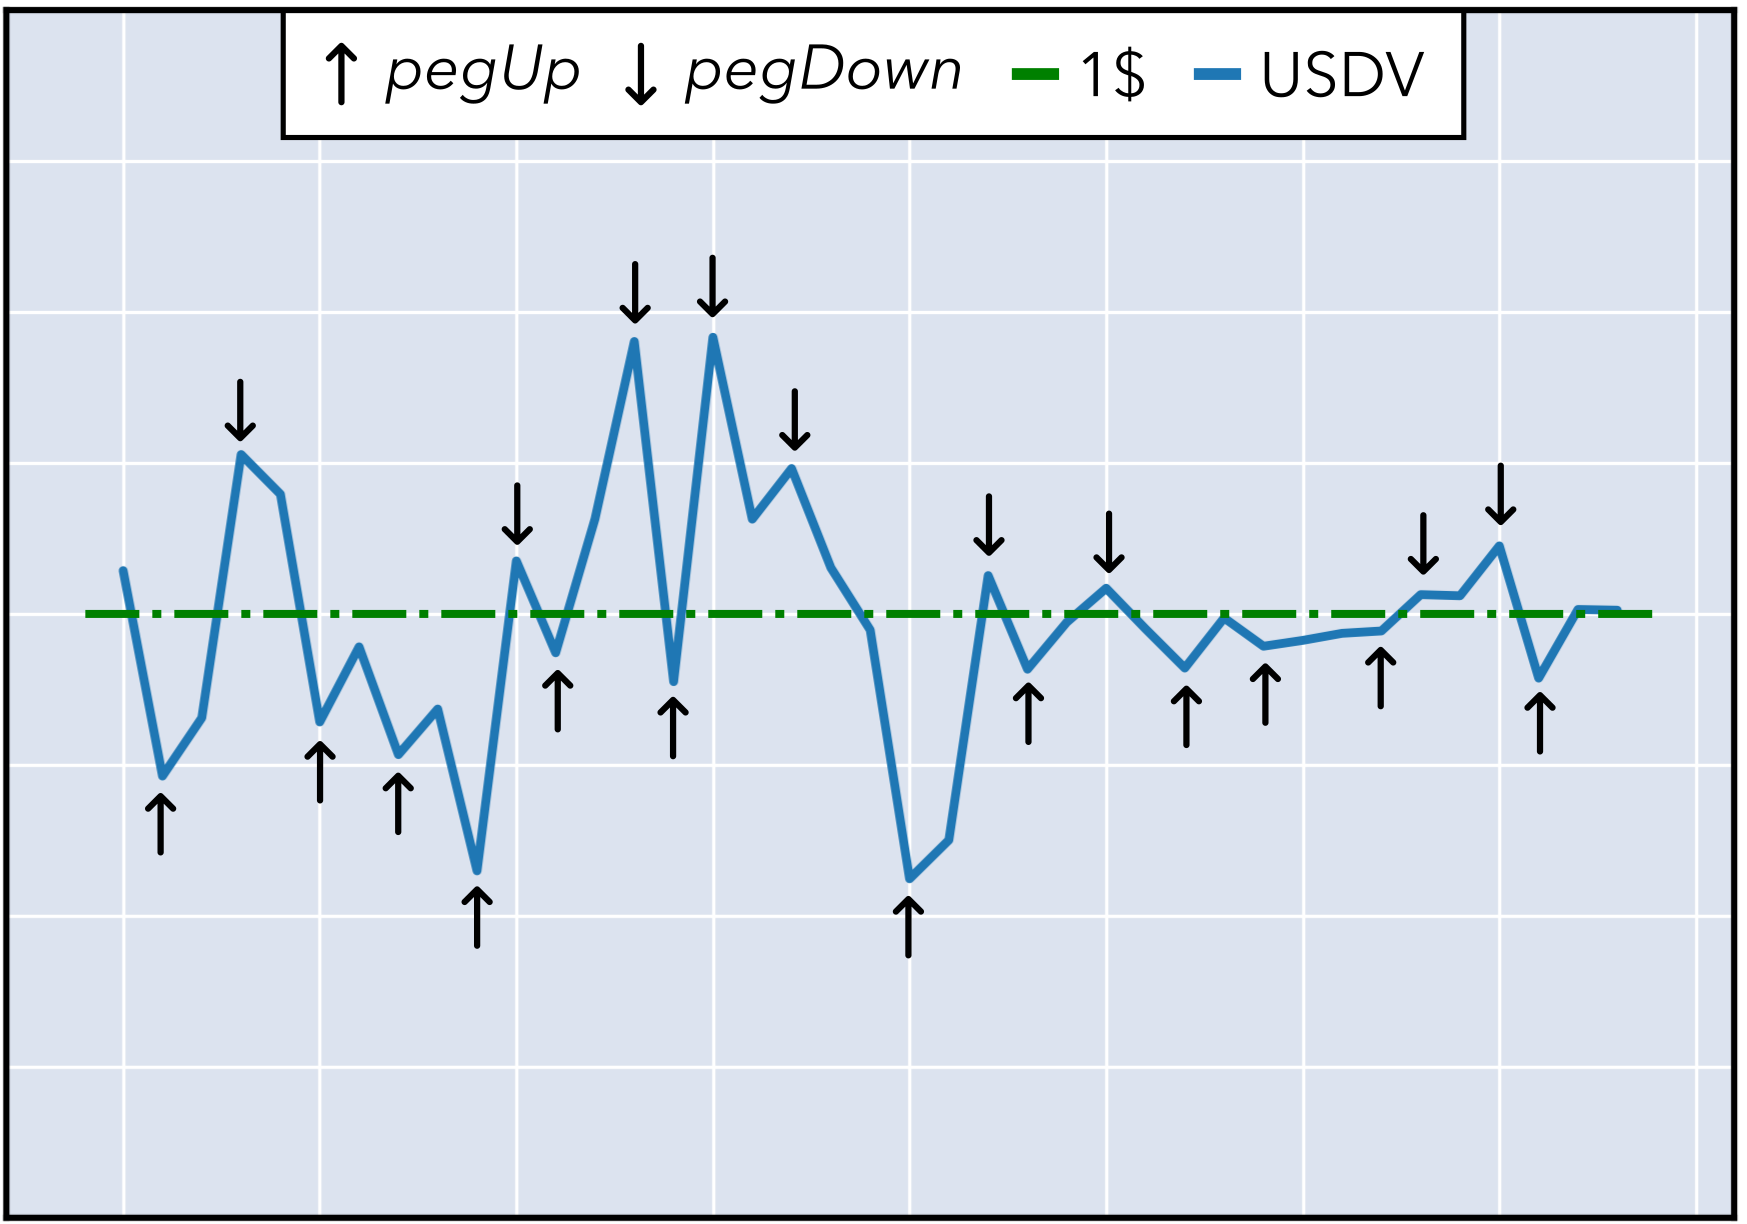
\includegraphics[width=0.8\textwidth]{figures/peg_stability.png}
    \vskip1em
    \caption{\usdv market scenario where its price (blue) is influenced by \textit{pegUp} ($\uparrow$) and \textit{pegDown} ($\downarrow$) events in order to stabilize the peg (green).}
    \label{fig:peg_stability}
\end{figure}

The \textit{pegUp} method is represented by an arrow up ($\uparrow$) and the \textit{pegDown} method is represented by an arrow down ($\downarrow$).
After an initiation phase, the \usdv peg can be successfully brought to balance by AE-PSM method calls.
The entire AE-PSM can furthermore be represented in a flow diagram as exemplified in Fig.\,\ref{fig:workflow}.
Here, a potential node runner or bot hits the entry point of the AE-PSM and obtains access to the \textit{pegUp} or \textit{pegDown} methods, that initiate either a burn process of \usdv (\textit{pegUp}) or a burn process of \vader (\textit{pegDown}) thus rebalancing the \usdv peg.

\vskip1em
\begin{figure}[ht!]
    \centering
    \begin{tikzpicture}[node distance = 2.5cm, auto]
        % Place nodes
        \node [aufpunkt] (psm) {PSM};
        \node [block, left of=psm] (xvader) {xVader};
        \node [cloud, above of=psm] (runner) {Node runner or bot};
        \node [block, below of=psm] (pool) {USDV 3pool};
        \node [block, right of=psm] (minter) {Vader minter};
        \node [block, right of=minter] (usdv) {USDV};
        \node [block, below of=usdv] (vader) {Vader};
        % Draw edges
        % PSM <-> xVader
        \draw[<-] (psm.west) -- node[rotate=60,above] {} (xvader.east);
        \draw[->] (psm.west) -- node[rotate=60,below] {} (xvader.east);
        % PSM <-> Aphra node runner
        \draw[->] (runner.south) -- node[xshift=0em] {$hit(amount)$} (psm.north);
        % PSM <-> USDV/3Pool
        \draw[->] (psm.south) -- node[rotate=60,above] {} (pool.north);
        \draw[->] (pool.north) -- node[rotate=60,below] {} (psm.south);
        % PSM <-> USDV/3Pool
        \draw[->] (psm.east) -- node[rotate=60,above] {} (minter.west);
        \draw[<-] (psm.east) -- node[rotate=60,below] {} (minter.west);
        % minter <-> USDV
        \draw[->] (minter.east) -- node[rotate=60,above] {} (usdv.west);
        \draw[<-] (minter.east) -- node[rotate=60,below] {} (usdv.west);
        % USDV <-> Vader
        \draw[->] (usdv.south) -- node[rotate=60,above] {} (vader.north);
        \draw[<-] (usdv.south) -- node[rotate=60,below] {} (vader.north);
    \end{tikzpicture}
    \vskip1em
    \caption{The AE-PSM is accessible through the \textit{hit} entry function that enables a bot or a node runner to interact with the module. If the \usdv peg is out of balance two events are available that decrease ($pegDown$) or increase ($pegUp$) the value of the \usdv stablecoin.}
    \label{fig:workflow}
\end{figure}
